\documentclass[12pt,leqno]{article}

\usepackage{indentfirst}

\usepackage{graphicx}
\graphicspath{ {./img/} }

\textwidth              16 cm
\textheight             23 cm
\oddsidemargin          -1 cm
\evensidemargin         -1 cm
\topmargin              -1 cm
\setlength{\evensidemargin}{15.5pt}
\setlength{\oddsidemargin}{2.5pt}

\pagestyle{empty}

\def\ClasaO{{\mathcal O}}

\usepackage{array}
\newcolumntype{P}[1]{>{\centering\arraybackslash}p{#1}}

\usepackage{multirow}
\usepackage{subcaption}
\usepackage{hyperref}

\usepackage{pgfplots}
\pgfplotsset{width=5in,compat=1.9}

\title{Two metaheuristic algorithms solving an optimization problem}
\author{Stamate Valentin 2B4}

\begin{document}

\maketitle

\section*{Abstract}
  This report contains the results of tow metaheristic algorithms solving an optimization
  problem. To have a better overview we will user tho diffent type of algorithms: a probabilistic
  one 'simulated annealing' and an evolutionary one a 'genetic algorithm'. Seeing the
  difference between these thwo we can make a better idea which one is bettwer. 

\section{Introduction}
  We already saw how these two types of algorithms work in the previous reports. Now, we
  can make them solve the same problem to see which one is better. The optimization problem
  to be solved is Asymetric Travelling Salesman Problem(ATSP). The algorithms are included
  in two different classes of metaheristic techniques: simulated annealing(SA) and genetic algorithm(GA).
  The main difference between these is that SA is a probalistic method and GA is inspired from evolution.
  10 instances will be used of ATSP to see what results they give on different inputs: br17, ftv33, ftv47, ft53, ftv70
  kro124, ftv170, rbg323, rbg358, rbg443. The temperature for SA is 100, and the number of iterations is 10000.
  The GA has a number of generation equal to 1000 and the population size is 400.
  
\subsection{Motivation}
  Both methods are good in finding an approximate solution. But which one? We know from previous
  raports that GA algorithms have more flexibility and we can make them fit better
  on different problems. SA on the other hand is less flexible so we may expect that
  GA is better.

\section{Methods}
  \subsection{Simulated Annealing}
    We initialize a random member and start the exploration. The solution has to be represented as a permutation
    that represents a Hamiltonian cycle. To be easier for us to find a neighbour, we will make a simple mutation with a codification based on OX Crossover
    like in our genetic algorithm. The start temperature is 100 and the stop temperature is $10^{-8}$ with a changind rate of 90\%. The number of iteration is 10000.
    
    The score is calculated as the cost of the Hamiltonian cycle. The fitness has the next formula: $fit(m) = 1 / m.score \cdot 1000$.
    
    The final result for all iterations is the smallest cost found.

  \subsection{Genetic Algorithm}
    When a member in the population is created the cromozome is randomly picked. This way
    we start with a population of 400 and for every generation we keep this number constant.
    Having the TSP, we have to find a way to encode a possible solution into a cromozome.
    A solution is represented as a permutation which is a cycle in the graph.
    So, a possible encoding can be the exact permutaion of the nodes. But, the problem is that 
    the corssover and mutation will be difficult to make.
    A better approach is to user OX Crossover, so we can apply the operators easily.
    The mutation can be made by incrementing the current gene modulo $n - 1 - i$ where i is the current position of the gene.
    
    There are three types of mutation. The first one is a greedy mutation and is applying 
    only if the fitness is better. The mutations probability is $10\%$ This operator is applied only for the first 10 members.
    The second one, is a mutation that is applied for the last 20 members and the increment number
    is randomly choose, so a part of the population will have more diversity. The last one is an adaptive normal mutation
    starting from $0.1\%$ to $2\%$.

    For every 10 generations, a normal mutation is applied to population just in case a wall is encountered.

    The score is simply the cost of the cycle, and the fitness is calculated this way: 
    $fit(m, minSc) = (pow(5.0, 1.0 / (m.sc - minSc + 10) + 2) - 25) * 100$ 
    where minSc, is the minimum score in the population.

    The selection is made by keeping only the best members.

    The number of generations is 1000.


\section{Experimental Setup}
  Each algorithm will be tested with 10 instances of ATSP. These are: br17, ftv33, ftv47, ft53, ftv70, kro124, ftv170, rbg323, rbg358, rbg443.
  \subsection*{Simulated Annealing}
  Number of iterations: 10000
  
  Start temperature: 100 | 90\% 
  
  End temperature: $10^{-8}$ 

  The sample size is 30.
  \subsection*{Genetic Algorithm}
  
  Number of generations: 1000
  
  Population size: 400
  
  Simple mutation probability: $0.1\% - 2\%$
  
  Greedy mutation probability: $10\%$

  Strong mutation probability: $40\%$
  
  The sample size is 30. \\


  Processor : Intel i5 - 8265U with 4 phisical and 8 virtual cores

  Compiler : TDM-GCC

\section{Results and Comparisons}

\begin{center}
  \begin{tabular}{|p{2.3cm}|p{2cm}||p{3cm}|p{2cm}|p{2cm}|p{2cm}|} 
    \hline
    \multicolumn{6}{|c|}{Simulated Annealing} \\
    \hline
    Instance      &  Expected  & Best Value & Mean & StDev & Duration \\ 
    \hline\hline
    br17          & $39$ & $ 206 $ & $ 238 $ & $ 14.39907 $ & 6min 33s \\ 
    \hline
    ftv33         & $1286$ & $ 4268 $ & $ 4396.3 $ & $ 73.17415 $ & 7min 23s \\ 
    \hline
    ftv47         & $ 1776 $ & $ 6913 $ & $ 6979.3 $ & $42.789$ & 13min 06s \\ 
    \hline
    ft53          & $6905$ & $ 24587 $ & $ 25356.6 $ & $ 461.0455 $ & 15min 16s \\ 
    \hline
    ftv70         & $1950$ & $ 9367 $ & $ 9687.4 $ & $123.0558 $ & 18min 33s \\ 
    \hline
    kro124        & $36230$ & $ 187001 $ & $ 194459 $ & $ 3228.695 $ & 26min 06s \\ 
    \hline
    ftv170        & $2755$ & $ 24436 $ & $ 24776.7 $ & $ 163.0741 $ & 36min 18s \\ 
    \hline
    rbg323        & $1326$ & $ 6152 $ & $ 6198.8 $ & $ 27.8799 $ & 1h 3m \\ 
    \hline
    rbg358        & $1163$ & $ 6791 $ & $ 6925.3 $ & $ 58.248 $ & 1h 12m \\ 
    \hline
    rbg443        & $2720$ & $ 8082 $ & $ 8169.26 $ & $ 41.859 $ & 1h 18m \\ 
    \hline
 \end{tabular}
\end{center}

\begin{center}
  \begin{tabular}{|p{2.3cm}|p{2cm}||p{3cm}|p{2cm}|p{2cm}|p{2cm}|} 
    \hline
    \multicolumn{6}{|c|}{Genetic Algorithm} \\
    \hline
    Instance      &  Expected  & Best Value & Mean & StDev & Duration \\ 
    \hline\hline
    br17          & $39$ & $ 39 $ & $ 39.3 $ & $ 0.48304 $ & 7min 46s \\ 
    \hline
    ftv33         & $1286$ & $ 1980 $ & $ 2041 $ & $ 26.969 $ & 8min 43s \\ 
    \hline
    ftv47         & $ 1776 $ & $ 3539 $ & $ 3554.1 $ & $47.7503$ & 18min 9s \\ 
    \hline
    ft53          & $6905$ & $ 15481 $ & $ 15495.7 $ & $ 10.1439 $ & 18min 32s \\ 
    \hline
    ftv70         & $1950$ & $ 5114 $ & $ 5114 $ & $ 0 $ & 26m 23s \\ 
    \hline
    kro124        & $36230$ & $ 102327 $ & $ 102327 $ & $ 0 $ & 42m 12s \\ 
    \hline
    ftv170        & $2755$ & $ 14915 $ & $ 15184.3 $ & $ 294.581 $ & 1h 06 \\ 
    \hline
    rbg323        & $1326$ & $ 3448 $ & $ 3547.5 $ & $ 74.723 $ & 3h 14m \\ 
    \hline
    rbg358        & $1163$ & $ 3839  $ & $ 3935.8 $ & $ 202.655 $ & 3h 43m \\ 
    \hline
    rbg443        & $2720$ & $ 4956 $ & $ 5024 $ & $ 77.661 $ & 4h 46m \\ 
    \hline
 \end{tabular}
\end{center}

Below is the cost evolution of the rbg323 input in one runtime.
\pagebreak

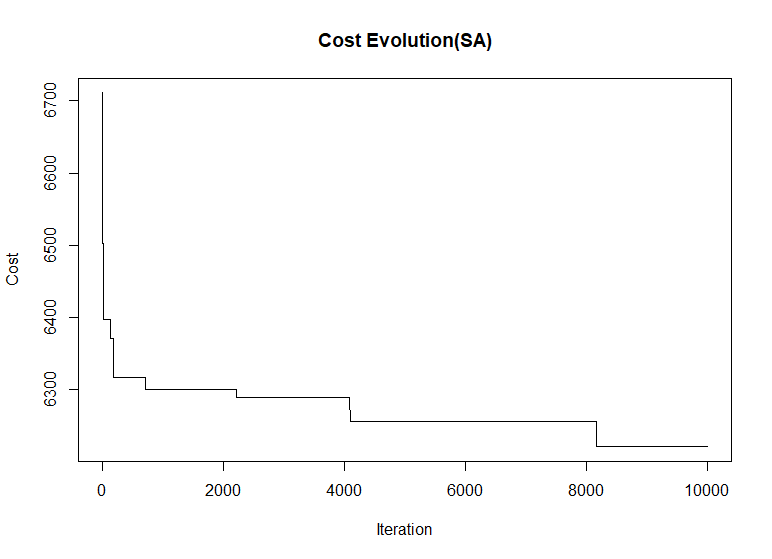
\includegraphics[width=0.9\linewidth]{sa.png} 

  Unlike the GA graph, the values remain constant for many iterations before a suddenly decrease.

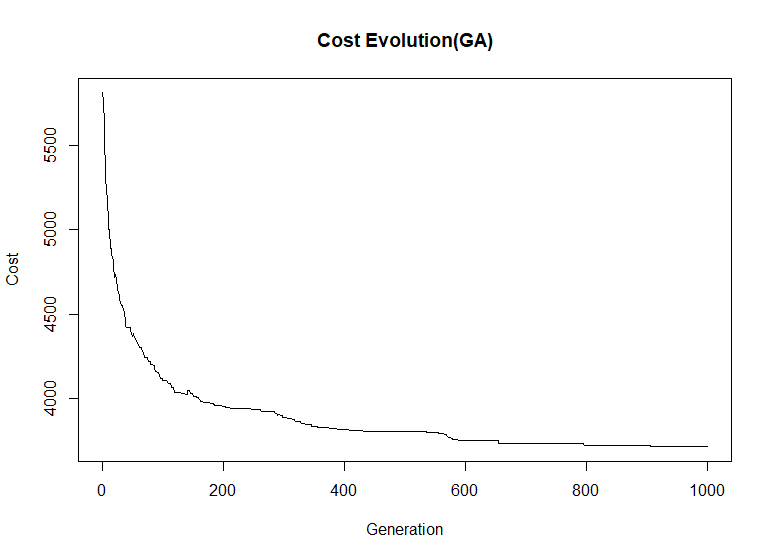
\includegraphics[width=0.9\linewidth]{ga.png} 

  The values are evolving like an inverse function and it's starting to decrease less between 600 and 1000 generations.

\pagebreak


\begin{center}
  \resizebox*{9cm}{9cm}{
    \begin{tikzpicture}
      \begin{axis}[
          title={Standar Deviation For SA},
          xlabel={Instance},
          ylabel={st-dev},
          xmin=1, xmax=10,
          ymin=0, ymax=3400,
          xtick={1, 2, 3, 4, 5, 6, 7, 8, 9, 10},
          ytick={0, 100, 3400},
          legend pos=north west,
          ymajorgrids=true,
          grid style=dashed,
      ]
      
      \addplot[
          color=blue,
          mark=square,
          ]
          coordinates {
          (1, 14)(2, 73)(3, 42)(4, 461)(5, 123)(6, 3228)(7, 163)(8, 27)(9, 58)(10, 41)
          };
          
      \end{axis}
    \end{tikzpicture}
  }  
\end{center}


\begin{center}
  \resizebox*{9cm}{9cm}{
    \begin{tikzpicture}
      \begin{axis}[
          title={Standar Deviation For GA},
          xlabel={Instance},
          ylabel={st-dev},
          xmin=1, xmax=10,
          ymin=0, ymax=300,
          xtick={1, 2, 3, 4, 5, 6, 7, 8, 9, 10},
          ytick={0, 100, 3400},
          legend pos=north west,
          ymajorgrids=true,
          grid style=dashed,
      ]
      
      \addplot[
          color=blue,
          mark=square,
          ]
          coordinates {
          (1, 0.4)(2, 26)(3, 47)(4, 10)(5, 0)(6, 0)(7, 294)(8, 74)(9, 202)(10, 77)
          };
          
      \end{axis}
    \end{tikzpicture}
  }  
\end{center}

Having these two graphs we can see what instances were 'harder' for each algorithm. For example, SA the kro124 instance is harder
but for GA the instances are ftv170 and rbg358.

\pagebreak

\section{Conclusions}
  We study the results given by two metaheuristic algorithms: simulated snnealing and a genetic algorithm solving a common
  hard problem: travelling salesman problem. We see what values each one gives as well as their evolution in one runtime.
  As we expected from the beginning, GA is bettwer than SA because it have more operators giving us more flexibilty. But, SA is good
  as well because is easier to implement and we should use it as a tradeof when it comes to result precision.


\begin{thebibliography}{9}
  \bibitem{}
    TSP problem: 
    \url{https://ro.wikipedia.org/wiki/Problema_comis-voiajorului}
    \bibitem{}

    Erase a vector: 
    \url{http://www.cplusplus.com/reference/vector/vector/erase/}
    \bibitem{}

    List STL: 
    \url{https://www.geeksforgeeks.org/list-cpp-stl/}
    \bibitem{}

    Random number generator: 
    \url{https://www.bitdegree.org/learn/random-number-generator-cpp}
    \bibitem{}

    TSP problem: 
    \url{https://www.geeksforgeeks.org/travelling-salesman-problem-set-1}
    \bibitem{}

    Undefined reference: 
    \url{https://stackoverflow.com/questions/16284629/undefined-reference-to-static-variable-c}
    \bibitem{}

    Array allocation: 
    \url{https://stackoverflow.com/questions/255612/dynamically-allocating-an-array-of-objects}
    \bibitem{}

    Static member: 
    \url{https://www.tutorialspoint.com/cplusplus/cpp_static_members.htm}
  \bibitem{}
    
    Laboratory site: 
    \url{https://profs.info.uaic.ro/~eugennc/teaching/ga/}
    \bibitem{}

    Instances: 
    \url{http://comopt.ifi.uni-heidelberg.de/software/TSPLIB95/}
    \bibitem{}

    Simulated annealing: 
    \url{https://en.wikipedia.org/wiki/Simulated_annealing}
    \bibitem{}

    Genetic algorithm: 
    \url{https://en.wikipedia.org/wiki/Genetic_algorithm}

  \end{thebibliography}  
  


\end{document}